\documentclass[12pt]{article}
\usepackage[left=1cm, right=1cm, top=2cm,bottom=1.5cm]{geometry} 

\usepackage[parfill]{parskip}
\usepackage[utf8]{inputenc}
\usepackage[T2A]{fontenc}
\usepackage[russian]{babel}
\usepackage{enumitem}
\usepackage[normalem]{ulem}
\usepackage{amsfonts, amsmath, amsthm, amssymb, mathtools}
\usepackage{tabularx}
\usepackage{hhline}

\usepackage{accents}
\usepackage{fancyhdr}
\pagestyle{fancy}
\renewcommand{\headrulewidth}{1.5pt}
\renewcommand{\footrulewidth}{1pt}

\usepackage{graphicx}
\usepackage[figurename=Рис.]{caption}
\usepackage{subcaption}
\usepackage{float}

%%Наименование папки откуда забирать изображения
\graphicspath{ {./images/} }

%%Изменение формата для ввода доказательства
\renewcommand{\proofname}{$\square$  \nopunct}
\renewcommand\qedsymbol{$\blacksquare$}

%%Изменение отступа на таблицах
\addto\captionsrussian{%
	\renewcommand{\proofname}{$\square$ \nopunct}%
}
%% Римские цифры
\newcommand{\RN}[1]{%
	\textup{\uppercase\expandafter{\romannumeral#1}}%
}

%% Для удобства записи
\newcommand{\MR}{\mathbb{R}}
\newcommand{\MQ}{\mathbb{Q}}
\newcommand{\MN}{\mathbb{N}}
\newcommand{\MTB}{\mathbb{T}}
\newcommand{\MI}{\mathrm{I}}
\newcommand{\MJ}{\mathrm{J}}
\newcommand{\MH}{\mathrm{H}}
\newcommand{\MT}{\mathrm{T}}
\newcommand{\MU}{\mathcal{U}}
\newcommand{\MV}{\mathcal{V}}
\newcommand{\MW}{\mathcal{W}}
\newcommand{\VN}{\varnothing}
\newcommand{\VE}{\varepsilon}

\theoremstyle{definition}
\newtheorem{defn}{Опр:}
\newtheorem{rem}{Rm:}
\newtheorem{prop}{Утв.}
\newtheorem{exrc}{Упр.}
\newtheorem{lemma}{Лемма}
\newtheorem{theorem}{Теорема}
\newtheorem{corollary}{Следствие}

\newenvironment{cusdefn}[1]
{\renewcommand\thedefn{#1}\defn}
{\enddefn}

\DeclareRobustCommand{\divby}{%
	\mathrel{\text{\vbox{\baselineskip.65ex\lineskiplimit0pt\hbox{.}\hbox{.}\hbox{.}}}}%
}
%Короткий минус
\DeclareMathSymbol{\SMN}{\mathbin}{AMSa}{"39}
%Длинная шапка
\newcommand{\overbar}[1]{\mkern 1.5mu\overline{\mkern-1.5mu#1\mkern-1.5mu}\mkern 1.5mu}
%Функция знака
\DeclareMathOperator{\sgn}{sgn}

%Функция ранга
\DeclareMathOperator{\rk}{\text{rk}}

%Обозначение константы
\DeclareMathOperator{\const}{\text{const}}

%Интеграл в большом формате
\DeclareMathOperator{\dint}{\displaystyle\int}
\newcommand{\ddint}[2]{\displaystyle\int\limits_{#1}^{#2}}

\newcommand{\smallerrel}[1]{\mathrel{\mathpalette\smallerrelaux{#1}}}
\newcommand{\smallerrelaux}[2]{\raisebox{.1ex}{\scalebox{.75}{$#1#2$}}}

\newcommand{\smallin}{\smallerrel{\in}}
\newcommand{\smallnotin}{\smallerrel{\notin}}

\newcommand*{\medcap}{\mathbin{\scalebox{1.25}{\ensuremath{\cap}}}}%
\newcommand*{\medcup}{\mathbin{\scalebox{1.25}{\ensuremath{\cup}}}}%

\makeatletter
\newcommand{\vast}{\bBigg@{3.5}}
\newcommand{\Vast}{\bBigg@{5}}
\makeatother

%Скалярное произведение
\DeclarePairedDelimiterX{\inner}[2]{\langle}{\rangle}{#1, #2}

%Подпись символов снизу
\newcommand{\ubar}[1]{\underaccent{\bar}{#1}}

%% Шапка для букв сверху
\newcommand{\wte}[1]{\widetilde{#1}}

\begin{document}
\lhead{Математический анализ - \RN{2}}
\chead{Шапошников С.В.}
\rhead{Лекция - 23}
\section*{Свойства интеграла Римана}

\begin{theorem}
	Пусть $f$ непрерывна на отрезке $[a,b]$, тогда функция $F(x) = \ddint{a}{x}f(t)dt$ дифференцируема на $[a,b]$ и $F^\prime(x) = f(x), \, \forall x \in [a,b]$. Тем самым, у всякой непрерывной функции есть первообразная.
\end{theorem}

\begin{corollary}
	Если $\widetilde{F}$ - первообразная функции $f$ на $[a,b]$, то справедлива формула Ньютона-Лейбница:
	$$
		\ddint{a}{b}f(t)dt = F(b) - F(a) = \widetilde{F}(b) - \widetilde{F}(a), \, \widetilde{F}(x) = F(x) + C, \, C \in \MR
	$$
\end{corollary}
\begin{proof}
	По формуле Ньютона-Лейбница:
	$$
		\widetilde{F}(b) - \widetilde{F}(a) = F(b) + C - F(a) - C = F(b) - F(a) = \ddint{a}{b}f(t)dt
	$$
	где $\widetilde{F}^\prime(x) = F^\prime(x) = f(x)$.
\end{proof}

\begin{corollary}(\textbf{Формула замены переменных})
	Пусть $f \in C[a,b]$, функция $\varphi \colon [\alpha,\beta] \to [a,b]$ (область значений функции $\varphi$ лежит в отрезке $[a,b]$, но не обязана совпадать) непрерывно дифференцируема. Тогда верно следующее равенство:
	$$
		\ddint{\alpha}{\beta}f\big(\varphi(t)\big){\cdot}\varphi^\prime(t)dt = \ddint{\varphi(\alpha)}{\varphi(\beta)}f(x)dx
	$$
\end{corollary}
\begin{proof}
	Возьмем любую первообразную функции $f = F^\prime$ (такая есть по предыдущей теореме). И воспользуемся формулой Ньютона-Лейбница несколько раз:
	$$
		\ddint{\varphi(\alpha)}{\varphi(\beta)}f(x)dx = F\big(\varphi(\beta)\big) - F\big(\varphi(\alpha)\big) = \ddint{\alpha}{\beta}\dfrac{d}{dt}F\big(\varphi(t)\big)dt = \ddint{\alpha}{\beta}f\big(\varphi(t)\big){\cdot}\varphi^\prime(t)dt 
	$$
\end{proof}
\begin{rem}
	Утверждение будет верным даже в том случае, если функция $f$ будет просто интегрируемой (см. упражнение в Зориче).
\end{rem}
\begin{corollary}(\textbf{Формула интегрирования по частям})
	Пусть $f,g$ - непрерывно дифференцируемы на отрезке $[a,b]$. Тогда верно следующее:
	$$
		\ddint{a}{b}f(x)g^\prime(x)dx = f(b)g(b) - f(a)g(a) - \ddint{a}{b}g(x)f^\prime(x)dx
	$$
\end{corollary}
\begin{proof}
	Заметим что по формуле Ньютона-Лейбница будет верно:
	$$
		\ddint{a}{b}\big(f(x)g(x)\big)^\prime dx = f(b)g(b) - f(a)g(a)
	$$
	Далее применим формулу Лейбница и линейность:
	$$
		\ddint{a}{b}\big(f(x)g(x)\big)^\prime dx = \ddint{a}{b}\big(f(x)g^\prime(x) + f^\prime(x)g(x)\big) dx = \ddint{a}{b}f(x)g^\prime(x) dx + \ddint{a}{b}f^\prime(x)g(x) dx = f(b)g(b) - f(a)g(a)
	$$
\end{proof}
\newpage
\section*{Формула Тейлора с остаточным членом в интегральной форме}
\begin{theorem}(\textbf{Формула Тейлора в интегральной форме})
	Пусть функция $f$ $(m+1)$-раз непрерывно дифференцируема в окрестности точки $a$, тогда:
	$$
		f(x) - f(a) = f^\prime(a)(x-a) + \dfrac{f^{\prime\prime}(a)(x-a)^2}{2!} + \dotsc + \dfrac{f^{(m)}(a)(x-a)^m}{m!} + r_m(a,x)
	$$
	где $r_m(a,x)$ - остаточный член в интегральной форме, который имеет следующий вид:
	$$
		r_m(a,x) = \dfrac{(-1)^m}{m!}\ddint{a}{x}(t-x)^mf^{(m+1)}(t)dt = \dfrac{1}{m!}\ddint{a}{x}(x-t)^mf^{(m+1)}(t)dt
	$$
\end{theorem}
\begin{proof}
	Пусть $x$ - фиксирован, тогда по формуле Ньютона-Лейбница и интегрированию по частям:
	$$
		f(x) - f(a) = \ddint{a}{x}1{\cdot}f^\prime(t)dt = \ddint{a}{x}(t-x)^\prime {\cdot}f^\prime(t)dt = (t-x){\cdot}f^\prime(t)\bigg|_{a}^{x} - \ddint{a}{x}(t-x){\cdot}f^{\prime\prime}(t)dt =
	$$
	$$
		 = f^\prime(a)(x-a) - \ddint{a}{x}(t-x){\cdot}f^{\prime\prime}(t)dt = f^\prime(a)(x-a) - \ddint{a}{x}\left(\dfrac{(t-x)^2}{2}\right)^\prime\!\!{\cdot}f^{\prime\prime}(t)dt =
	$$
	$$
		= f^\prime(a)(x-a) - \dfrac{f^{\prime\prime}(t)(t-x)^2}{2!}\bigg|_a^x + \ddint{a}{x}\dfrac{(t-x)^2}{2}{\cdot}f^{\prime\prime}(t)dt = f^\prime(a)(x-a) +  \dfrac{f^{\prime\prime}(a)(x-a)^2}{2!} + \ddint{a}{x}\dfrac{(t-x)^2}{2}{\cdot}f^{\prime\prime}(t)dt
	$$
	Продолжаем интегрировать по частям, на шаге $m$ получим:
	$$
		f(x) - f(a) = \displaystyle\sum\limits_{k=1}^m \dfrac{f^{(k)}(a)(x-a)^k}{k!} + \dfrac{(-1)^m}{m!}\ddint{a}{x}(t-x)^m{\cdot}f^{(m+1)}(t)dt
	$$
\end{proof}
\begin{rem}
	В выражении остаточного члена сделаем замену $t = a + s(x-a) \Rightarrow dt = (x-a)ds$, границы интегрирования изменятся с $[a,x]$ на $[0,1]$ и $t-x = a - x + s(x-a) = - (x - a)(1 - s)$. Тогда получим:
	$$
		r_m(a,x) = \dfrac{(-1)^m}{m!}\ddint{a}{x}(t-x)^mf^{(m+1)}(t)dt = \dfrac{(-1)^m}{m!}\ddint{0}{1}(-1)^m (x-a)^m (1-s)^m f^{(m+1)}\big(a + s(x-a)\big)(x-a)ds = 
	$$
	$$
		= \dfrac{(x-a)^{m+1}}{m!}\ddint{0}{1}(1-s)^mf^{(m+1)}\big(a + s(x-a)\big)ds
	$$
\end{rem}
На практике почти всегда применяется данная теорема для разложения функции в ряд Тейлора.
\begin{exrc}
	Вывести формулу Тейлора с остаточным членом в форме Лагранжа, применяя аналог теоремы о среднем (первую теорему о среднем для интеграла).
\end{exrc}
\begin{theorem}(\textbf{Первая теорема о среднем для интеграла})
	Пусть $f, g$ и их произведение $fg$ интегрируемы на отрезке $[a,b]$, пусть имеются точная нижняя и верхняя грани функции $f$: 
	$$
		m = \inf\limits_{[a,b]}f(x), \, M = \sup\limits_{[a,b]}f(x)
	$$ 
	Если функция $g$ неотрицательна (или неположительна) на отрезке $[a,b]$, то будет верно:
	$$
		\ddint{a}{b}(fg)(x)dx = \mu \ddint{a}{b}g(x)dx
	$$
	где $\mu \in [m,M]$. Если также известно, что $f \in C[a,b]$, то найдется точка $\xi \in [a,b]$ такая, что:
	$$
		\ddint{a}{b}(fg)(x)dx = f(\xi)\ddint{a}{b}g(x)dx
	$$
\end{theorem}
\begin{proof}
	Пусть $a < b$ и пусть $g(x) \geq 0$ на $[a,b]$. Поскольку у функции $f$ имеются точная нижняя и верхняя грани, то при $g(x) \geq 0$ получим:
	$$
		mg(x) \leq f(x)g(x) \leq Mg(x)
	$$
	Тогда по линейности и по монотонности получим:
	$$
		m\ddint{a}{b}g(x)dx \leq \ddint{a}{b}f(x)g(x)dx \leq M\ddint{a}{b}g(x)dx
	$$
	Если $\ddint{a}{b}g(x)dx = 0$, то требуемое выполнено. Если $\ddint{a}{b}g(x)dx \neq 0$, то полагая:
	$$
		\mu = \left(\ddint{a}{b}g(x)dx\right)^{-1}\!\!{\cdot}\ddint{a}{b}(fg)(x)dx
	$$
	мы получим, что $m \leq \mu \leq M$ и требуемое равенство выполнено. В случае если функция $f \in C[a,b]$, то по теореме о промежуточном значении $\exists \, \xi \in [a,b]\colon f(\xi) = \mu$.
\end{proof}
\begin{theorem}(\textbf{Формула Тейлора с остаточным членом в форме Лагранжа})
	Пусть $f$ $(m+1)$-раз непрерывно дифференцируема в окрестности точки $a$, тогда:
	$$
		f(x) - f(a) = f^\prime(a)(x-a) + \dfrac{f^{\prime\prime}(a)(x-a)^2}{2!} + \dotsc + \dfrac{f^{(m)}(a)(x-a)^m}{m!} + r_m(a,x)
	$$
	где $r_m(a,x)$ - остаточный член в форме Лагранжа, который имеет следующий вид:
	$$
		r_m(a,x) = \dfrac{f^{(m+1)}(\xi)(x - a)^{m+1}}{(m+1)!}
	$$
\end{theorem}
\begin{proof}
	В условиях теоремы о формуле Тейлора в интегральной форме мы знаем, что:
	$$
		f(x) - f(a) = f^\prime(a)(x-a) + \dfrac{f^{\prime\prime}(a)(x-a)^2}{2!} + \dotsc + \dfrac{f^{(m)}(a)(x-a)^m}{m!} +  \dfrac{1}{m!}\ddint{a}{x}(x-t)^mf^{(m+1)}(t)dt
	$$
	Рассмотрим остаточный член подробнее: 
	\begin{enumerate}[label={(\arabic*)}]
		\item функция $f^{(m+1)}(t)$ - непрерывна на $[a,x]$ по условию, следовательно достигает на отрезке своей точной нижней и верхней грани ($m$ и $M$ соответственно);
		\item функция $g(t) = (x-t)^m$ - непрерывна на $[a,x]$ и неотрицательна;
		\item произведение этих функций - непрерывно на $[a,x]$ и следовательно интегрируемо на нём;
	\end{enumerate}
	Таким образом, по первой теореме о среднем для интеграла найдется $\xi \in [m,M]$ такое, что:
	$$
		\dfrac{1}{m!}\ddint{a}{x}(x-t)^mf^{(m+1)}(t)dt = \dfrac{f^{(m+1)}(\xi)}{m!}\ddint{a}{x}(x-t)^mdt = -\dfrac{f^{(m+1)}(\xi)}{(m+1)!}{\cdot}(x-t)^{m+1}\bigg|_{t=a}^x = \dfrac{f^{(m+1)}(\xi)(x-a)^{m+1}}{(m+1)!}
	$$
\end{proof}
\begin{corollary}
	Пусть $f \colon \MR^n \to \MR$ $(m+1)$ раз дифференцируема в окрестности точки $a$, тогда для достаточно малых $h$ будет выполнено:
	$$
		f(a + h) - f(a)  =  \displaystyle\sum\limits_{k=1}^m \dfrac{1}{k!}d^mf(a,h) + \dfrac{1}{m!}\ddint{0}{1}(1-s)^m{\cdot}d^{m+1}f(a + sh, h)ds
	$$
\end{corollary}
\begin{proof}
	Рассмотрим функцию $\varphi(t) = f(a+th)$ и применим к ней теорему:
	$$
		\varphi(1) - \varphi(0) = \displaystyle\sum\limits_{k=1}^m\dfrac{\varphi^{(m)}(0)}{k!} + \dfrac{1}{m!}\ddint{0}{1}(1-s)^m{\cdot}\varphi^{(m+1)}(s)ds
	$$
	Как мы знаем $\varphi^{(k)}(t) = d^kf(a+ th,h)$, подставим это в выражение и получим требуемое:
	$$
		f(a+t) - f(a) = \displaystyle\sum\limits_{k=1}^m\dfrac{d^mf(a,h)}{k!} + \dfrac{1}{m!}\ddint{0}{1}(1-s)^m{\cdot}d^{m+1}f(a + sh, h)ds
	$$
\end{proof}

\newpage
\section*{Частные случаи формулы Тейлора в интегральной форме}
Формула Тейлора с остаточным членом в интегральной форме - это очень удобная форма записи функции и в ряде частных случаев она позволяет достаточно кратко получить интересные следствия.
\begin{corollary}(\textbf{Лемма Адамара})
	Пусть $f \colon \MR^n \to \MR$ - непрерывно дифференцируема в окрестности нуля и $f(0) = 0$. Тогда существуют непрерывные в окрестности $0$ функции $g_k(x)$ такие, что:
	$$
		f(x) = \displaystyle \sum\limits_{k = 1}^n x_k {\cdot} g_k(x)	
	$$
\end{corollary}
\begin{proof}
	Пусть $a = 0, \, a + h = x$, применяем формулу Тейлора при $m = 0$ и тогда получим:
	$$
		f(x) - f(0) = f(x) = \ddint{0}{1}(1-s)^0{\cdot}d^{0+1}f(sx,x)ds = \ddint{0}{1}df(sx,x)ds = \ddint{0}{1}\sum\limits_{k=1}^{n}\dfrac{\partial f}{\partial x_k}(sx){\cdot}x_k ds
	$$
	Воспользовавшись тем, что интеграл это линейная функция, мы получим следующее выражение:
	$$
		f(x) = \sum\limits_{k=1}^n x_k{\cdot}\ddint{0}{1}\dfrac{\partial f}{\partial x_k}(sx) ds = \sum\limits_{k = 1}^{n}x_k{\cdot}g_k(x)
	$$
	Рассмотрим модуль разности функции $g_k(x)$ и воспользуемся теоремой о среднем:
	$$
		|g_k(x) - g_k(y)| = \left|\ddint{0}{1}\dfrac{\partial f}{\partial x_k}(sx) ds  - \ddint{0}{1}\dfrac{\partial f}{\partial x_k}(sy) ds\right| \leq \max\limits_{s \smallin [0,1]}\left| \dfrac{\partial f}{\partial x_k}(sx) - \dfrac{\partial f}{\partial x_k}(sy) \right|
	$$
	где последнее неравенству верно в силу того, что значение функции в некоторой точке $c \in [0,1]$ находится между точной нижней и верхней гранью. Рассмотрим разность по норме:
	$$
		\|sx - sy\| = |s|{\cdot}\|x - y\| \leq \|x - y\|
	$$
	Возьмем замкнутый шар $\overline{B}(0,r)$ вокруг точки $0$ на котором $\tfrac{\partial f}{\partial x_k}$ - непрерывная и будем брать точки $x,y$ только внутри этого шара. Непрерывная функция на компакте - равномерно непрерывна (по теореме Кантора). Тогда: 
	$$
		\forall \VE > 0, \, \exists \, \delta > 0 \colon \forall x,y \in \overline{B}(0,r), \, \|x - y\| < \delta \Rightarrow \max\limits_{s \smallin [0,1]}\left| \dfrac{\partial f}{\partial x_k}(sx) - \dfrac{\partial f}{\partial x_k}(sy) \right| < \VE \Rightarrow |g_k(x) - g_k(y)| < \VE
	$$
\end{proof}
При $n =1$, лемма Адамара говорит о том, что если $f(0) = 0$, то: 
$$
	f(x) = x{\cdot}g(x)
$$ 
Это напоминает теорему Безу: 
$$
	f(x) = (x - 0){\cdot}g(x) = x{\cdot}g(x)
$$ 
При $n = 2$, лемма Адамара говорит о том, что если $f(0,0) = 0$, то: 
$$
	f(x_1,x_2) = x_1{\cdot}g_1(x) + x_2{\cdot}g_2(x)
$$ 
Таким образом в одномерном случае можно поделить на $x$ и доказать требуемое, но в многомерном случае так сделать уже не получится.
\begin{corollary}
	Пусть $f\colon \MR^n \to \MR$ - дважды непрерывно дифференцируема в окрестности $0$, функция и её градиент принимают следующие значения: $f(0) = 0, \, \nabla f(0) = 0$. Тогда существуют непрерывные в окрестности $0$ функции $g_{k,m}$ такие, что:
	$$
		f(x) = \sum\limits_{k,m}x_kx_mg_{km}(x)
	$$
\end{corollary}
\begin{exrc}
	Доказать следствие (указание: необходимо применить формулу Тейлора для $m = 1$).
\end{exrc}
\begin{proof}
	Пусть $a = 0, \, a + h = x$, применяем формулу Тейлора при $m = 1$ и тогда получим:
	$$
		f(x) = df(0)(x-0) + \dfrac{1}{2}\ddint{0}{1}(1-s){\cdot}d^{2}f(sx,x)ds = \dfrac{1}{2}\ddint{0}{1}(1-s){\cdot}\sum\limits_{k,m}\dfrac{\partial^2 f}{\partial x_k \partial x_m}(sx){\cdot}x_k{\cdot}x_m ds 
	$$
	Поскольку $f(0) = 0, \, \nabla f(0) = 0$. Воспользовавшись тем, что интеграл это линейная функция, мы получим следующее выражение:
	$$
		f(x) = \dfrac{1}{2}\sum\limits_{k,m} x_k{\cdot}x_m{\cdot}\ddint{0}{1}(1-s)\dfrac{\partial^2 f}{\partial x_k \partial x_m}(sx) ds = \sum\limits_{k,m}x_k{\cdot}x_m{\cdot}g_{k,m}(x)
	$$
	Рассмотрим модуль разности $|g_{k,m}(x) - g_{k,m}(y)|$ и воспользуемся теоремой о среднем (произведение непрерывных функций - непрерывная):
	$$
		\left|\ddint{0}{1}(1-s)\dfrac{\partial^2 f}{\partial x_k \partial x_m}(sx) ds  - \ddint{0}{1}(1-s)\dfrac{\partial^2 f}{\partial x_k \partial x_m}(sy) ds\right| \leq \max\limits_{s \smallin [0,1]}(1-s){\cdot}\left| \dfrac{\partial^2 f}{\partial x_k \partial x_m}(sx) - \dfrac{\partial^2 f}{\partial x_k \partial x_m}(sy) \right|
	$$
	где последнее неравенству верно в силу того, что значение функции в некоторой точке $c \in [0,1]$ находится между точной нижней и верхней гранью. Рассмотрим разность по норме:
	$$
		\|sx - sy\| = |s|{\cdot}\|x - y\| \leq \|x - y\|
	$$
	Возьмем замкнутый шар $\overline{B}(0,r)$ вокруг точки $0$ на котором $\tfrac{\partial^2 f}{\partial x_k \partial x_m}$ - непрерывная и будем брать точки $x,y$ только внутри этого шара. Непрерывная функция на компакте - равномерно непрерывна (по теореме Кантора). Поскольку $\forall x \in \overline{B}(0,r) \Rightarrow sx \in \overline{B}(0,r), \, \forall s \in [0,1]$, то тогда: 
	$$
		\forall \VE > 0, \, \exists \, \delta > 0 \colon \forall x,y \in \overline{B}(0,r), \, \|x - y\| < \delta \Rightarrow \|sx - sy\| < \delta \Rightarrow
	$$
	$$
		\Rightarrow \max\limits_{s \smallin [0,1]}(1-s){\cdot}\left| \dfrac{\partial^2 f}{\partial x_k \partial x_m}(sx) - \dfrac{\partial^2 f}{\partial x_k \partial x_m}(sy) \right| < \VE {\cdot} \max\limits_{s \smallin [0,1]}(1-s) = \VE \Rightarrow |g_{k,m}(x) - g_{k,m}(y)| < \VE
	$$
\end{proof}
Первое утверждение дает функции вида: 
$$
	a_1x_1 + \dotsc + a_n x_n
$$ 
то есть линейные функции в окрестности $x$ с зависящими от $x$ коэффициентами $a_1,\dotsc, a_n$. Второе утверждение дает функции вида:
$$
	\displaystyle \sum\limits_{k,m}x_k x_m a_{km}
$$ 
то есть квадратичные функции опять же с зависящими от $x$ коэффициентами. 

Данные результаты можно сравнить с тем, о чем утверждала теорема о неявной функции: если производная невырождена (хотя бы по одной переменной $x_k$), то можно ввести координаты, где функция будет линейной. Следствие же утверждает, что если мы не знаем ничего про вырожденность производной, то тоже можем записать функцию, не меняя координаты, почти как линейную.

Есть теорема похожая на теорему о неявной функции, которая утверждает, что если первые производные вырождаются, при этом матрица вторых производных невырождена, то в правильной системе координат функция будет квадрикой.
\begin{theorem}(\textbf{Лемма Морса})
	Пусть $f$ - трижды непрерывно дифференцируема в окрестности точки $x = 0$ и $f(0) = 0, \, \nabla f(0) = 0$. Пусть матрица $\left(\tfrac{\partial^2 f}{\partial x_i \partial x_j}(0)\right)_{i,j}$ - невырождена. Тогда существует диффеоморфизм $x = \varphi(u)$ окрестности нуля на окрестность нуля такой, что верно следующее:
	$$
		f\big(\varphi(u) \big) = u_1^2 + \dotsc + u_r^2	- u_{r+1}^2 - \dotsc -u_n^2, \, 0 \leq r \leq n
	$$
\end{theorem}
\begin{proof}
	По предыдущему следствию получим:
	$$
		f(x) = \sum\limits_{k,m}x_k{\cdot}x_m{\cdot}g_{km}(x), \, g_{km}(x) = \dfrac{1}{2} \ddint{0}{1}(1-s)\dfrac{\partial^2 f}{\partial x_k \partial x_m}(sx) ds
	$$
	где $g_{km}$ - непрерывно дифференцируемые (без доказательства, утверждение из следующего семестра). Значение этих функций в точке $0$ следующее (в силу единственности разложения Тейлора):
	$$
		g_{km}(0) = \dfrac{1}{2}\ddint{0}{1}\dfrac{\partial^2 f}{\partial x_k \partial x_m}(0) ds = \dfrac{1}{2}\dfrac{\partial^2 f}{\partial x_k \partial x_m}(0)
	$$
	Тогда матрица из этих функций $g_{km}$ - симметрична $\Rightarrow$ можно привести квадратичную форму этой матрицы к главным осям (нормальной форме). Обозначим матрицу вторых производных $(g_{km}) =G$. Сделаем линейную замену координат $x = Cy$, тогда:
	$$
		\widetilde{f}(y) = f(Cy) = x^T G x\big|_{x = Cy} = y^T C^T G C y = y^T \widetilde{G} y = \sum\limits_{k,m}\widetilde{g}_{km}(y)y_ky_m, \,  \widetilde{G}  = C^T G C
	$$
	Рассмотрим следующую квадратичную форму с матрицей $G(0)$:
	$$
		\sum\limits_{k,m}g_{km}(0)x_k x_m 
	$$
	Так как $G(0)$ - невырождена, то существует $C$ такая, что её можно привести к нормальному виду (то есть можно привести $G(0)$ к диагональному виду):
	$$
		\sum\limits_{k,m}\widetilde{g}_{km}(0)y_ky_m = y_1^2 + \dotsc + y_r^2 - y_{r+1}^2 - \dotsc - y_n^2	
	$$
	Таким образом, в одной точке функция уже имеет правильный вид. Функции $g_{k,m}$ непрерывны, поэтому мало отличаются от своих значений в нуле $\Rightarrow$ с точностью до погрешности функция уже имеет требуемый вид, необходимо избавиться от погрешности сделав нелинейную замену.
	
	Пусть $\widetilde{g}_{11}(0) = 1$ (может быть $-1$). Следовательно рядом с $0$ значение функции $\wte{g}_{11}$ будет положительным числом (можно извлечь корень). Соберем все слагаемые, где имеется $y_1$ и выделим полный квадраты:
	$$
		\wte{g}_{11}y_1^2 + 2\wte{g}_{12}y_1 y_2 + \dotsc + 2 \wte{g}_{1n}y_1 y_n = \left(\sqrt{\wte{g}_{11}}y_1 + \dfrac{\wte{g}_{12}}{\sqrt{\wte{g}_{11}}} y_2 + \dotsc + \dfrac{\wte{g}_{1n}}{\sqrt{\wte{g}_{11}}} y_n \right)^2 - \dfrac{\wte{g}_{12}^2}{\wte{g}_{11}} y_2^2 - \dotsc - \dfrac{\wte{g}_{1n}^2}{\wte{g}_{11}} y_n^2
	$$
	Нужно отметить, что данное выражение в $0$ будет равно $y_1^2$ (все слагаемые, кроме первого, будут $0$). Подставим такое разложение в функцию $\wte{f}(y)$ и сгруппируем слагаемые, тогда получим:
	$$
		\wte{f}(y) = \left(\sqrt{\wte{g}_{11}}y_1 + \dfrac{\wte{g}_{12}}{\sqrt{\wte{g}_{11}}} y_2 + \dotsc + \dfrac{\wte{g}_{1n}}{\sqrt{\wte{g}_{11}}} y_n \right)^2 + \sum\limits_{k,m \geq 2}\widehat{g}_{km}y_ky_m
	$$
	Заметим, что в точке $0$ ничего не изменится, поскольку $\wte{G}(0)$ - диагональная, то есть:
	$$
		\sum\limits_{k,m \geq 2}\widehat{g}_{km}(0)y_ky_m = y_2^2 + \dotsc + y_r^2 - y_{r+1}^2 - \dotsc - y_n^2
	$$
	Сделаем следующую замену:
	$$
		\varphi_1(y) \colon u_1 = \sqrt{\wte{g}_{11}}y_1 + \dfrac{\wte{g}_{12}}{\sqrt{\wte{g}_{11}}} y_2 + \dotsc + \dfrac{\wte{g}_{1n}}{\sqrt{\wte{g}_{11}}} y_n, \, u_2 = y_2, \dotsc, \, u_n = y_n
	$$
	Подставляя замену, мы получим следующий вид функции $\wte{f}$:
	$$
		\wte{f}(u) = u_1^2 + \sum\limits_{k,m \geq 2}\widehat{g}_{km}(u)u_k u_m
	$$
	Проверим, что эта замена локально явлется диффеоморфизмом и далее утверждение будет верно по индукции. Рассмотрим матрицу Якоби этой замены в нуле (по теореме об обратной функции):
	$$
		J_{\varphi_1}(0) = 
		\begin{pmatrix}
			\dfrac{\partial u_1}{\partial y_1}(0) & * & * & \dotsc & * \\
			* & 1 & 0 & \dotsc & 0 \\
			* & 0 & 1 & \dotsc & 0 \\
			* & \vdots & \vdots & \ddots & \vdots \\
			* & 0 & 0 & \dotsc & 1
		\end{pmatrix} \Rightarrow |J_{\varphi_1}(0)| = \dfrac{\partial u_1}{\partial y_1}(0) = \sqrt{\wte{g}_{11}(0)}{\cdot}1 + 0 + \dotsc + 0 = \sqrt{\wte{g}_{11}(0)} = 1 > 0
	$$
	где в производной все слагаемые с $y_i$ равны $0$ (поскольку $y_i =0 ,\, \forall i = \overline{1,n}$ в точке $0$). И таким образом, замена локально является диффеоморфизмом (по теореме об обратной функции). По остальным переменным - аналогично.
\end{proof}

Одним из применений леммы Морса может быть анализ динамических систем в $\MR^2$. 

\textbf{Пример}: Пусть $F \colon \MR^2 \to \MR, \, F = C, \, F(0) = 0, \, \nabla F(0) = 0$, тогда система в ``равновесии'' будет иметь один из следующих видов:
$$
	x^2 + y^2 = C, \, x^2 - y^2 = C
$$

\newpage
\section*{Критерии интегрируемости по Риману}
До настоящего момента самым важным утверждением являлось следующее:
$$
	\ddint{a}{b}F^\prime(x)dx = F(b) - F(a)
$$
где $F^\prime$ - непрерывная. Все полезные следствия до настоящего момента мы выводили из него. Но вообще-то, по условию, это равенство верно, когда $F^\prime$ является интегрируемой. Если хотим пользоваться этой формулой, чтобы по производной восстанавливать первообразную при ослаблении условий, что $F^\prime$ - непрерывна, необходимо научиться в первую очередь проверять, когда $F^\prime$ - интегрируема.

До сих пор мы владели только достаточным условием: если мы умеем приближать функцию ступенчатой, то она будет интегрируемой.

\begin{theorem}(\textbf{Необходимое условие интегрируемости по Риману})
	Если $f$ интегрируема по Риману на отрезке $[a,b]$, то $f$ - ограничена на отрезке $[a,b]$.
\end{theorem}
\begin{proof}
	Пусть $\VE =1$, тогда:
	$$
		\exists \, \delta > 0 \colon \forall (\MTB, \xi), \, \lambda(\MTB) < \delta \Rightarrow \left|\ddint{a}{b}f(x)dx - \sigma(f, \MTB, \xi)\right| < \VE = 1
	$$
	Раскроем модуль:
	$$
		\ddint{a}{b}f(x)dx - 1 <\sigma(f, \MTB, \xi) = \sum\limits_{k = 1}^N f(\xi_k){\cdot}|\Delta_k| < \ddint{a}{b}f(x)dx + 1
	$$
	Фиксируем $\xi_2,\dotsc, \xi_N$, рассмотрим отрезок $\Delta_1$ и получим оценку на $f(\xi_1)$ для любой точки на нём:
	$$
		\forall \xi_1 \in \Delta_1, \, C_3 < f(\xi_1) < C_2	
	$$
	Таким образом, функция $f$ ограничена на $\Delta_1$. Аналогичным образом, так можно проделать для каждого отрезка $\Delta_k \Rightarrow f$ ограничена на каждом отрезке $\Delta_k \Rightarrow f$ ограничена на отрезке $[a,b]$, который из них составлен.
\end{proof}

Далее нам понадобится более продвинутый инструментарий в интегрируемости, возникающий в теории сумм Дарбу, которую можно считать альтернативным способом построения интеграла Римана (более геометрическим).
\newpage
\section*{Суммы и интегралы Дарбу}
Всегда предполагаем, что $f$ - ограничена на изучаемом отрезке.
\begin{defn}
	$\forall$ разбиения $\MTB$ отрезка $[a,b]$ следующая сумма:
	$$
		s(f,\MTB) = \sum\limits_{k = 1}^N \inf\limits_{\Delta_k}f{\cdot}|\Delta_k| 
	$$
	называется \uwave{нижней суммой Дарбу}.
\end{defn}
\textbf{\uline{Геометрический смысл}}: Нижняя сумма Дарбу представляет из себя площадь вписанных под график функции прямоугольников (Римановы суммы могут накладываться на график).
\begin{defn}
	$\forall$ разбиения $\MTB$ отрезка $[a,b]$ следующая сумма:
	$$
		S(f,\MTB) = \sum\limits_{k = 1}^N \sup\limits_{\Delta_k}f{\cdot}|\Delta_k| 
	$$
	называется \uwave{верхней суммой Дарбу}.
\end{defn}
\textbf{\uline{Геометрический смысл}}: Верхняя сумма Дарбу представляет из себя площадь описывающих график функции прямоугольников (по самой верхней точке графика на соответствующих отрезках).

\begin{figure}[H]
	\centering
	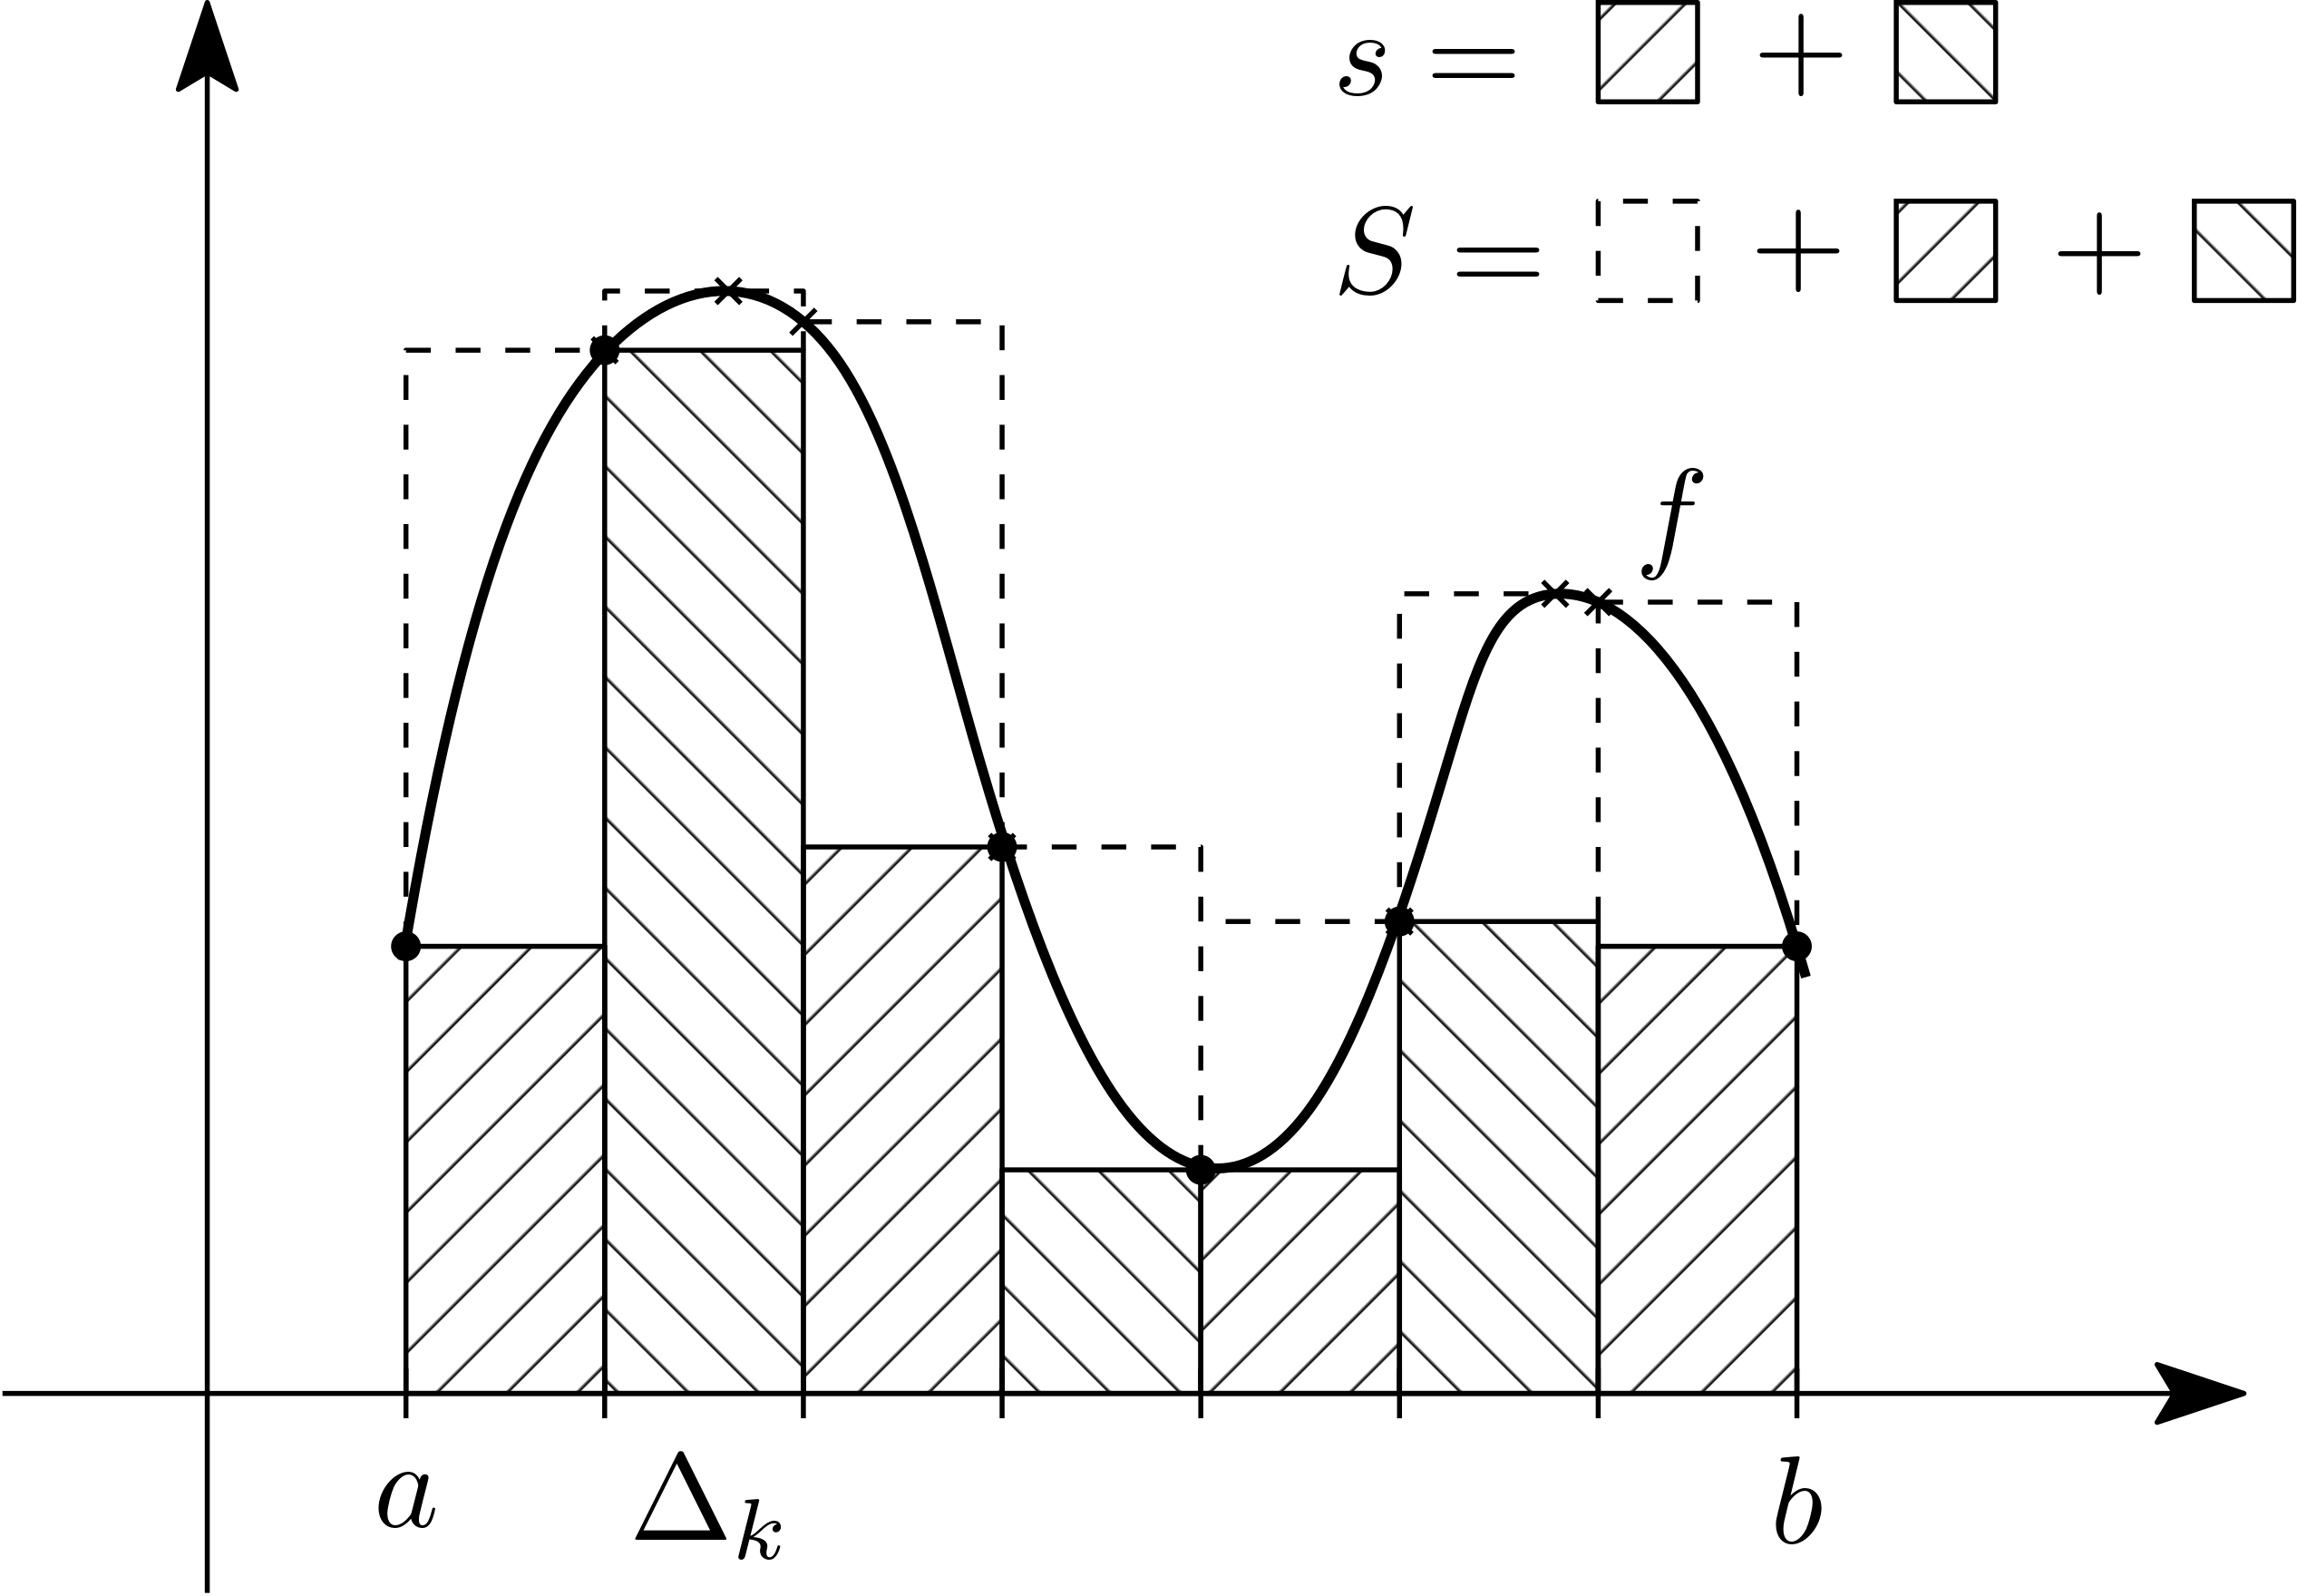
\includegraphics[width=0.5\textwidth]{23_1.png}
	\label{23_1}
	\caption{Геометрический смысл сумм Дарбу.}
	\label{fig:Суммы Дарбу}
\end{figure}

Интуитивно, функция интегрируема если площадь фигур под графиком и над графиком в пределе совпадают. 

\textbf{Пример}: Функция Дирихле:
$$
	D(x) = 
	\begin{cases}
		1, & x \in \MQ\\
		0, & x \notin \MQ
	\end{cases}
$$ 
Тогда $s = 0$, а $S = 1$ и сближения никакого не будет (функция Дирихле не интегрируема).

Чем лучше эти суммы, чем Римановы суммы? В суммах Дарбу нет отмеченных точек,  выбор точек определен.

\begin{lemma}
	Верны следующие утверждения:
	\begin{enumerate}[label={(\arabic*)}]
		\item $s(f,\MTB) = \inf\limits_{\xi}\sigma(f,\MTB,\xi) \leq \sigma(f,\MTB,\xi) \leq \sup\limits_{\xi}\sigma(f,\MTB,\xi) = S(f,\MTB)$;
		\item Пусть $\MTB \subset \MTB^\prime$ (измельчение разбиения $\MTB$), тогда $s(f,\MTB) \leq s(f,\MTB^\prime)$ и $S(f,\MTB) \geq S(f,\MTB^\prime)$;
		\item $\forall \, \MTB_1, \MTB_2, \, s(f,\MTB_1) \leq S(f,\MTB_2)$;
	\end{enumerate}
\end{lemma}
\begin{proof}\hfill
	\begin{enumerate}[label={(\arabic*)}]
		\item $\forall \xi, \, s(f,\MTB) \leq \sigma(f,\MTB,\xi)$ поскольку $\inf\limits_{\Delta_k}f \leq f(\xi_k)$. Возьмем $\VE > 0$, тогда по определению точной нижней грани получим:
		$$
			\exists \, \xi_k \in \Delta_k \colon f(\xi_k) < \inf\limits_{\Delta_k}f + \VE
		$$
		Умножим на $\Delta_k$ и просуммируем такие неравенства по $k$, получим следующее:
		$$
			\sigma(f,\MTB,\xi) < s(f,\MTB) + \VE(b-a) \Rightarrow \inf\limits_\xi \sigma(f,\MTB,\xi) < s(f,\MTB) + \VE(b-a)
		$$
		Устремляя $\VE$ к нулю, получим:
		$$
			\inf\limits_\xi \sigma(f,\MTB,\xi) \leq s(f,\MTB)
		$$
		А поскольку $\forall \xi, \, s(f,\MTB) \leq \sigma(f,\MTB,\xi)$, то:
		$$
			s(f,\MTB) \leq \inf\limits_\xi\sigma(f,\MTB,\xi) \Rightarrow s(f,\MTB) = \inf\limits_\xi \sigma(f,\MTB,\xi)
		$$
		Аналогичные рассуждения проводятся для $S(f,\MTB)$ и получим требуемое неравенство;
		\item Возьмем разбиение $\MTB^\prime$ (состоит из отрезков $\Delta^\prime$), которое размельчает разбиение $\MTB$ (состоит из отрезков $\Delta$), то есть $\MTB \subset \MTB^\prime$. Можно считать, что:
		$$
			\Delta_k = \bigcup\limits_{i = 1}^{m_k} \Delta_k^i, \, \Delta_k^i \subset \Delta^\prime
		$$
		Рассмотрим слагаемое нижней суммы дарбу на интервале $\Delta_k$ и распишем $\Delta_k$ в сумму $\Delta_k^i$:
		$$
			\inf\limits_{\Delta_k}f{\cdot}|\Delta_k| = \sum\limits_{i = 1}^{m_k}\inf\limits_{\Delta_k}f{\cdot}|\Delta_k^i|
		$$
		Точная нижняя грань функции $f$ на части $\Delta_k^i$ большего интервала $\Delta_k$, будет не меньше, чем на самом $\Delta_k$, тогда:
		$$
			\inf\limits_{\Delta_k}f \leq \inf\limits_{\Delta_k^i}f
			\Rightarrow \sum\limits_{i = 1}^{m_k}\inf\limits_{\Delta_k}f{\cdot}|\Delta_k^i| \leq \sum\limits_{i = 1}^{m_k}\inf\limits_{\Delta_k^i}f{\cdot}|\Delta_k^i|
		$$
		Просуммируем неравенства по $k$ и получим:
		$$
			\sum\limits_{k = 1}^{N}\inf\limits_{\Delta_k}f{\cdot}|\Delta_k| = s(f,\MTB) =  \sum\limits_{k = 1}^{N}\sum\limits_{i = 1}^{m_k}\inf\limits_{\Delta_k}f{\cdot}|\Delta_k^i| \leq \sum\limits_{k = 1}^{N}\sum\limits_{i = 1}^{m_k}\inf\limits_{\Delta_k^i}f{\cdot}|\Delta_k^i| = s(f,\MTB^\prime)
		$$
		Аналогичные рассуждения проводятся для верхней суммы Дарбу;
		\item Пусть имеются два разбиения $\MTB_1, \MTB_2$, составим из них новое разбиение, состящее из всех точек этих: $\MTB_1 \cup \MTB_2$. Новое разбиение будет измельчением как $\MTB_1$, так и $\MTB_2$. Тогда по предыдущему пункту леммы получим:
		$$
			s(f,\MTB_1) \leq s(f,\MTB_1 \cup \MTB_2) \leq S(f,\MTB_1 \cup \MTB_2) \leq S(f,\MTB_2)
		$$
		И таким образом, мы получили требуемое;
	\end{enumerate}
\end{proof}
Благодаря этой лемме мы понимаем, что нижние суммы Дарбу ограничены сверху, а верхние - снизу, следовательно точная верхняя грань нижних сумм и точная нижняя грань верхних сумм Дарбу - конечны.
\begin{defn}
	Точная верхняя грань нижней суммы Дарбу:
	$$
		\sup\limits_{\MTB}s(f,\MTB) = \underline{\MI}
	$$
	называется \uwave{нижним интегралом Дарбу}.
\end{defn}

\textbf{\uline{Геометрический смысл}}: Вписываем фигуры под график и берем их супремум, тогда $\underline{\MI}$ должен приближать площадь под графиком снизу.

\begin{defn}
	Точная нижняя грань верхней суммы Дарбу:
	$$
	\inf\limits_{\MTB}S(f,\MTB) = \overline{\MI}
	$$
	называется \uwave{верхним интегралом Дарбу}.
\end{defn}

\textbf{\uline{Геометрический смысл}}: Описываем фигуры над графиком (так чтобы включалась область под ним) и берем их инфинум, тогда $\overline{\MI}$ должен приближать площадь под графиком сверху.

\begin{theorem}(\textbf{Критерий Дарбу})
	Функция $f$ интегрируема по Риману $\Leftrightarrow  \overline{\MI} = \underline{\MI}$.
\end{theorem}

\end{document}